\chapter{Micropost Annotation}
\label{cha:micropost-annotation}

% the code below specifies where the figures are stored
\ifpdf
    \graphicspath{{4_micropost_annotation/figures/PNG/}{4_micropost_annotation/figures/PDF/}{4_micropost_annotation/figures/}}
\else
    \graphicspath{{4_micropost_annotation/figures/EPS/}{4_micropost_annotation/figures/}}
\fi

\section{Introduction}

For the task of making sense out of social network microposts,
our contributions are methods to consolidate and rank
the results of multiple named-entity recognition and
disambiguation Web services that we have unified in form
of a~wrapper Web service that (i) takes care of both
consolidation and ranking, and that
(ii) transparently tracks the underlying Web services'
data provenance.

According to official statistics, Facebook is the biggest
social network with one billion monthly active
users\footnote{\url{http://newsroom.fb.com/Key-Facts},
accessed November 20, 2012}
as of October 2012.
Official user statistics from
Twitter\footnote{\url{http://blog.twitter.com/2012/03/twitter-turns-six.html},
accessed November 20, 2012}
stemming from March 2012 suggest
that currently more than 140 million active users
share 340 million tweets a~day.
Altogether, the users of social networks
produce an incredible amount of public and private data.
In this chapter, we thus report on methods to access and make sense
out of \emph{public} status updates,
or, our preferred term, microposts.

\subsection{Direct Access to Micropost Raw Data}

Social networks in general offer so-called
Application Programming Interfaces (APIs)
in order to allow for developers to access
part of the networks' data programmatically.
Similar to the microblogging site Twitter
with its search
API\footnote{\url{https://dev.twitter.com/docs/api/1.1/get/search/tweets},
accessed November 20, 2012},
Facebook offers both a~search function on the website,
and a~search
API\footnote{\url{https://developers.facebook.com/docs/reference/api/},
accessed November 20, 2012},
and so does
\googleplus\footnote{\url{https://developers.google.com/+/api/},
accessed November 20, 2012}.
In order to perform data mining,
a~statistically significant amount of microposts is necessary.
Having access to \emph{all} microposts of a~service is referred to as
having access to the \emph{fire hose}.
Typically, developers are only granted access to a~smaller random 
sample of microposts (colloquially referred to as \emph{garden hose} access).
While Twitter grants all developers \emph{garden hose} access to its Streaming
APIs\footnote{\url{https://dev.twitter.com/docs/streaming-apis},
accessed November 20, 2012},
for Facebook and \googleplus there are no such documented options.

\subsection{Browser Extensions to Access Microposts Indirectly}

To address this shortage, we have developed browser extensions
for the two major social networks Facebook and Twitter,
called Facebook Swarm
NLP\footnote{\url{http://bit.ly/facebookswarmnlp},
accessed November 20, 2012}
and Twitter Swarm
NLP\footnote{\url{http://bit.ly/twitterswarmnlp},
accessed November 20, 2012},
for a~popular Web browser.
These extensions inject JavaScript code into Facebook and
Twitter to perform data analysis on the encountered set of
\emph{public} microposts by sending extracted data
to a~central data processing unit.
Users need to be logged in to Facebook or Twitter for the 
extensions to work, and must have given
their \emph{explicit agreement} during
the extension installation process
for part of their data being shared in an anonymized way.
While this is far inferior and not comparable at all
with direct \emph{fire hose} access,
given a~critical amount of participants,
it still provides access to a~random sample of microposts
from different social networks.

\subsection{Data Analysis Flow}

The extensions first retrieve all status updates
from the contacts that are displayed
on the current user's timeline.
Second, the extensions perform named-entity extraction (NEE)
and disambiguation via Natural Language Processing (NLP)
using a~remote NLP API on each of the microposts
in order to add semantic meaning to them.
The extracted named entities are then displayed
along each micropost, as illustrated in \autoref{fig:facebook}.
Finally the extracted named entities
are sent to a~central Web analytics framework~\cite{kaushik2009analytics}
to compute basic or advanced trends, for example,
by ranking the most discussed-about named entities per day,
or by pivoting named entities by Web analytics data,
like users' geographic locations.

\begin{figure}[htb!]
  \centering
  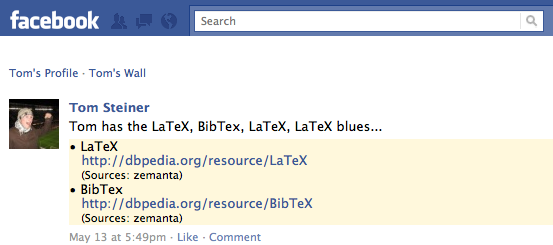
\includegraphics[width=0.75\textwidth]{facebook-swarm-nlp.png}
  \caption[Facebook Swarm NLP browser extension]
    {Facebook Swarm NLP browser extension.
    Extracted named entities have a~pale yellow background.}     
  \label{fig:facebook}
\end{figure}

\subsection{A~Wrapper API for Named-Entity Disambiguation}

As mentioned before, in order to perform named-entity extraction
and disambiguation, we rely on a~wrapper API
that calls existing third-party NLP APIs in the background
and that delivers the combined results of these APIs
in a~consolidated way.
It is  desirable
(i)~to credit back the contribution of each single third-party API
to the joint results, and
(ii)~to track the provenance of the joint results
in order to understand how they were formed.
We will show how these two constraints
can be fulfilled in a~generalizable way
at the concrete example of the wrapper NLP API
used for our browser extensions.

\section{Related Work}

We regard related work from different angles.
First, we look into different approaches
for named-entity disambiguation,
which is relevant for adding meaning to microposts.
Second, we look into efforts in mashing up Web services,
which is important for tracking data provenance
when using multiple APIs in combination.

\subsection{Entity Disambiguation Using Lexical Databases}

In~\cite{choudhury2009youtubetags},
Choudhury \emph{et al.}\ describe a~framework for
semantic enrichment, ranking, and integration
of Web video tags using Semantic Web technologies.
This task is more related to microposts
than it seems at first sight:
video tags can consist of more than one word,
and microposts (especially on Twitter) oftentimes consist
of just a~few words.
In order to enrich the typically sparse
user-generated tag space,
meta data like the recording time and location
or the video title and video description are used,
but also social features such as the playlists
where a~video appears in and related videos.
Next, the tags are ranked by their co-occurrence
and in a~final step interlinked to DBpedia~\cite{auer2007dbpedia}
concepts for greater integration with other datasets.
The authors disambiguate the tags based on
WordNet~\cite{miller1995wordnet,fellbaum1998wordnet}
synsets (groups of data elements that are considered
semantically equivalent for the purposes of information retrieval)
if possible, \emph{i.e.},
if there is only one matching synset in WordNet,
the corresponding WordNet URI in DBpedia is selected.
If there are more than one matching synsets,
the tags' and their context tags' similarity is computed
to decide on an already existing tag URI.

\subsection{Entity Disambiguation with Semantic Coherence and News Trends}

In~\cite{fernandez2007identityrank},
Fernández \emph{et al.}\ examine named-entity disambiguation
in the context of news annotation.
Their approach consists of three steps:
finding the candidate instances in the NEWS
ontology~\cite{fernandez2010newsontology}
for each entity in a~news item,
ranking these candidate instances
using a~modified version of
PageRank~\cite{brin1998pagerank},
and finally retraining the algorithm
with the journalist's feedback once the process is finished.
The approach first takes into account the number
of occurrences of candidate entities in the past
in order to find news trends,
and second, the occurrences of candidate entities
in past articles in the same categories
in order to find semantic coherences.

\subsection{Disambiguation with Disambiguation Dictionaries}

In~\cite{nguyen2008namedentity},
Nguyen \emph{et al.}\ show how disambiguation dictionaries
can be used to disambiguate entities
using Wikipedia disambiguation pages.
For a~set of entity candidates, all disambiguations are ranked
using tf--idf (or cosine similarity)~\cite{manning2008ir}.
The approach is a~hybrid and incremental process
that utilizes previously identified named entities
and related terms co-occurring with ambiguous names
in a~text for entity disambiguation.

\subsection{Disambiguation with Corpuses and Probability}

Cucerzan shows in~\cite{cucerzan2007largescale}
the use of a~corpus like Wikipedia for entity disambiguation.
The surrounding words of the to-be-disambiguated terms
plus the tags and categories of the related Wikipedia articles
are used to determine semantic coherence and thus
to decide on the most probable entity candidate.
This happens through a~process of heuristically maximizing
the agreement between contextual information
extracted from Wikipedia and the context of a~document.

\subsection{Disambiguation With Search Query Logs}

In~\cite{billerbeck2010rankingentities}, Billerbeck \emph{et al.}\
use click graphs and session graphs
of users' search engine sessions
to semantically bridge different queries in order to
retrieve entities for a~concrete entity retrieval query.
Click graphs are created by using queries and URLs as nodes
and connecting and weighting them by their click frequencies.
Session graphs are created by using only queries as nodes
with edges between them if they appear in the same user sessions,
again weighted by co-occurrence frequencies.
An exemplary entity retrieval query is \emph{hybrid cars},
semantically bridgeable queries are then \emph{toyota prius},
or \emph{honda civic hybrid}).
These entities are then ranked and returned to the user.

\subsection{Combining Different Web Services and Provenance}

In~\cite{groth2009mashups}, Groth \emph{et al.}\
describe how so-called mash-ups can be created in a~dynamic,
just-in-time way, combining data from different data sources
through tools and technologies such as
Yahoo! Pipes\footnote{\url{http://pipes.yahoo.com/pipes/},
accessed November 20, 2012},
RSS~\cite{cadenhead2006rss}, and APIs.
The authors are driven by the motivation to allow for trust
and confidence in mash-ups, and therefore
consider it critical to be able to analyze the origin
of combined results.
They suggest an approach based on OWL~\cite{mcguinness2004owl}
and XML~\cite{bray2008xml},
with a~focus on process documentation.
However, different from our work, where the goal is to transparently
add provenance data at API invocation time,
their focus is more on overall process documentation
in the context of a~mash-up application.

The focus of Carroll \emph{et al.}\ in~\cite{carroll2005namedgraphs}
is on the provenance of triples in the Semantic Web world, namely,
for making statements about triples in graphs.
Therefore, the authors introduce the concept of Named Graphs,
an extension to RDF~\cite{klyne2004rdf}.
In contrast to our work, Carroll \emph{et al.}\
focus purely on using triples to make statements about triples
(\emph{i.e.}, stay in the RDF world),
whereas our approach uses RDF to make statements
about potentially any API result.
 
Web service specifications in the context of the 
first-generation standards represented by WSDL~\cite{christensen2001wsdl},
SOAP~\cite{gudgin2007soap}, and UDDI~\cite{sabbouh2001uddi}
are occasionally referred to collectively as \emph{WS--*}.
In the \emph{WS--*} world, BPEL4WS, described by
Curbera \emph{et al.}\ in~\cite{curbera2003bpel4ws}
provides a~formal language for the specification of
business processes and business interaction protocols.
This allows for the combination of several APIs.
However, it does not credit back concrete outputs of a~combined API
to the underlying APIs.

\section{Structuring Unstructured Textual Data} 
\label{sec:structuring}

When we speak of adding structure to unstructured textual data,
we mean the process of extracting the main concepts
in the form of named entities from a~given text
and the process of disambiguating those named entities,
\emph{i.e.}, the removal of uncertainty of meaning from
an ambiguous named entity like \emph{Barcelona},
which can stand for the football club, or the city of Barcelona.
An \emph{entity} is defined by
WordNet~\cite{miller1995wordnet,fellbaum1998wordnet}
as \textit{``that which is perceived or known or inferred
to have its own distinct existence (living or nonliving)''}. 
Typically, named entities from a~text can be persons, companies,
organizations, geographies, but also things like quantities,
expressions of time, books, albums, authors, \emph{etc.}
The extraction of named entities is commonly based on
Natural Language Processing (NLP) combined with Machine Learning.

\subsection{Natural Language Processing Services}
\label{sec:nlp-services}

WordNet~\cite{miller1995wordnet,fellbaum1998wordnet}
defines \emph{Natural Language Processing} as
\textit{``the branch of information science that deals with
natural language information''}.
From the many NLP toolkits available,
hereafter, we list some NLP Web services
that link to datasets in the
Linking Open Data
cloud~\cite{bizer2011statelodcloud,cyganiak2011lodcloud}
in order to disambiguate named entities.

\subsubsection{OpenCalais}\label{sec:opencalais}

The
OpenCalais\footnote{\url{http://www.opencalais.com/documentation/opencalais-documentation},
accessed November 20, 2012}
Web service automatically creates rich semantic metadata
for textual documents.
Using Natural Language Processing (NLP),
machine learning and other methods, OpenCalais analyzes documents
and finds the entities within and also returns the facts and
events hidden within them.
OpenCalais is the only of the examined Web services
that provides details on occurrences in concrete sections
of the submitted coherent text.
This allows for the exact matching of the location in the text
where a~certain entity is believed to appear.
This is especially useful as OpenCalais
is also oftentimes capable of recognizing references
within the text to prior discovered entities
(for example, in the following text,
\emph{he} is mapped back to Obama: \textit{``\emph{Obama}
thanked people for their work in ensuring the victory.
\emph{He} also thanked his family.''}).
An OpenCalais response consists of three parts:

\begin{itemize}
  \item a~list of topics that the text is categorized in.
  \item a~list of concrete entities that occur in the text.
  \item a~list of social concept tags.
\end{itemize}

The problem with the extracted entities is
that they are not always uniquely disambiguated.
An example is the URL \url{http://d.opencalais.com/pershash-1/cf42394f-4ae9-3e8e-958a-088149c86565.html}
that represents the concept of an entity of type \texttt{person}
named \emph{Barack Hussein Obama}.
However, a~\texttt{person}-type \emph{Barack Obama} entity from the same document is also represented by the URL
\url{http://d.opencalais.com/pershash-1/cfcf1aa2-de05-3939-a7d5-10c9c7b3e87b.html}
Other services successfully disambiguated both occurrences and
recognized them to stand for the same person, President Obama.
A~second issue is that only a~tiny fraction of the returned
entities link to other Linked Open Data sources in the
LOD cloud~\cite{bizer2011statelodcloud,cyganiak2011lodcloud}.
In order to discover links to the LOD cloud,
each returned entity URL has to be retrieved at the expense
of an HTTP request, and the returned RDF has to be checked
for said links.

\subsubsection{AlchemyAPI}

AlchemyAPI\footnote{\url{http://www.alchemyapi.com/api/entity/},
accessed November 20, 2012}
is capable of identifying people, companies, organizations,
cities, geographic features, and other typed entities within
textual documents.
The service employs statistical algorithms and NLP
to extract semantic richness embedded within text.
AlchemyAPI differentiates between entity extraction and
concept tagging.
AlchemyAPI's concept tagging API is capable of abstraction, \emph{i.e.},
understanding how concepts relate and tag them accordingly
(``Hillary Clinton'', ``Michelle Obama'', and ``Laura Bush" are all
tagged as ``First Ladies of the United States'').
In practice, the difference between named-entity extraction
and concept tagging is subtle.
In consequence, we treat entities and concepts the same.
Overall, AlchemyAPI results are very accurate
and in the majority of cases excellently interlinked
to well-known members of the LOD cloud,
among others with DBpedia~\cite{auer2007dbpedia},
OpenCyc~\cite{lenat1995cyc},
and Freebase~\cite{markoff2007freebase}.
AlchemyAPI also provides links to other data sources, however,
sometimes the returned URLs result in \texttt{404 Not found}.
One example that we came across during our tests was the URL
\url{http://umbel.org/umbel/ne/wikipedia/George\_W.\_Bush.rdf}, which should represent the concept of the person George W. Bush.
The URL does serve as a~Semantic Web identifier, however, 
harms the third Linked Data principle,
as outlined in \autoref{sec:linked-data-principles}.
AlchemyAPI also oftentimes returns thematically closely related,
but for a~concrete text not directly relevant entities
beyond the abstract concepts from its concept tagging service,
for example, in a~text about the CEO of a~given company, a~CEO of one of its competitors, but that is not directly mentioned in the text.

\subsubsection{Zemanta}

Zemanta\footnote{\url{http://developer.zemanta.com/docs/},
accessed November 20, 2012}
allows developers to query the service for contextual metadata
about a~given text.
The returned components currently span four categories:
articles, keywords, photos, in-text links, and
optional component categories.
The service provides high quality entities that are linked
to well-known datasets of the LOD cloud, \emph{e.g.},
DBpedia or Freebase.
Zemanta convinces through very accurate entity disambiguation
and thus high precision, however, at the cost of recall.
Where other services return named entities of lower precision,
the design objectives of Zemanta instead seem to prefer
not to return anything at all.

\subsubsection{DBpedia Spotlight}

DBpedia Spotlight~\cite{mendes2011dbpediaspotlight}
is a~tool for annotating mentions of DBpedia resources in text,
providing a~solution for linking unstructured information sources
to the Linked Open Data cloud through DBpedia.
DBpedia Spotlight performs named-entity extraction,
including entity detection and disambiguation
with adjustable precision and recall.
DBpedia Spotlight allows users to configure the annotations
to their specific needs through the DBpedia
Ontology\footnote{\url{http://wiki.dbpedia.org/Ontology},
accessed November 20, 2012}
and quality measures such as prominence, topical pertinence,
contextual ambiguity and disambiguation confidence.

\subsection{Machine Translation}
\label{sec:machine-translation}

Social networking happens at a~global scale.
In consequence, many microposts are authored
in languages different from English.
In order to still make sense out of those microposts,
we apply machine translation to translate non-English microposts
to English.
We use the Google Translate
API\footnote{\url{https://developers.google.com/translate/v2/getting_started},
accessed November 21, 2012}
which, if the source language parameter is left blank,
tries to first detect the source language,
and subsequently translates the micropost to English.

\subsection{Part-of-Speech Tagging}
\label{sec:part-of-speech-tagging}

Our processing chain supports part-of-speech (POS) tagging
based on a~Brill POS tagger~\cite{brill1992pos} adapted for JavaScript.
Brill taggers work by assigning tags to each word and then changing them
using a~set of predefined rules.
In an initial run, if a~word is known, the tagger
first assigns the most frequent tag,
or, if a~word is unknown, it naively assigns the tag ``noun'' to it.
By applying over and over the processing rules and
changing the incorrect tags, a~sufficiently high accuracy is achieved.
In the current processing chain, POS tagging does not yet
play an active role,
however, we aim for leveraging the additional data
for better micropost analysis in the future.

\section{Consolidating Named-Entity Disambiguation Results} 
\label{sec:consolidate}

In this section, we motivate the use of multiple
named-entity disambiguation Web services in \emph{parallel}
with the objective of obtaining named entity candidates
for a~textual document such as a~micropost.
The task of evaluating and aligning named-entity extraction and
disambiguation APIs and their typed output
has been formally addressed by Rizzo \emph{et al.}\
in the context of the NERD
framework~\cite{rizzo2011nerd,rizzo2012nerd}.
We have decided for a~type-agnostic approach,
which we motivate in the following.

\subsection{Identity Links on the Semantic Web}
\label{sec:sameasorg}

From the considered services, only OpenCalais returns data in its
own namespace (\url{http://d.opencalais.com/*}), which is
weakly, however, not in all cases,
interlinked with other datasets in the LOD cloud.
In contrast, the other services return results either directly
in the DBpedia namespace (\url{http://dbpedia.org/resource/*}),
as in the case of DBpedia Spotlight,
or in the DBpedia namespace together with other
well interlinked LOD cloud dataset namespaces, like Freebase
(\url{http://rdf.freebase.com/rdf/*}) in the cases of
AlchemyAPI and Zemanta.

In order to address the problem of different namespaces in results,
an approach as presented by Glaser \emph{et al.}\ 
in~\cite{glaser2009sameas} based on \texttt{owl:sameAs} links
could be used.
In practice, however, while many resources in the Linked Data
world are marked as equivalent to each other,
the quality of such equivalence links is not always excellent.
An example of a~good equivalence link is shown in \autoref{code:sameas}.

\begin{lstlisting}[caption={Example of a~good equivalence link},
  label={code:sameas},
  escapechar=§]
<http://dbpedia.org/resource/Barack_Obama> §\linewrap§
  <http://www.w3.org/2002/07/owl#sameAs> §\linewrap§
  <http://rdf.freebase.com/rdf/en.barack_obama> .
\end{lstlisting}

\noindent As Halpin \emph{et al.}\ show
in a~study~\cite{halpin2010owlsameas}, the problem
with \texttt{owl:sameAs} is that people tend to use it
in different ways with different intentions.
In~\cite{halpin2010owlsameas},
the authors differentiate between four separate usage styles,
ranging from expressing loose relatedness,
to strict equivalence.
Despite the different intentions, people tend to incorrectly use
\texttt{owl:sameAs} habitually, according to the study.
Inference is thus problematic, if not impossible,
when the intention of the link creator of the particular
\texttt{owl:sameAs} link is unknown.

\subsection{Linked Data Principles Applied}

We recall the Linked Data principles, as outlined
in \autoref{sec:linked-data-principles}.
In order to represent extracted named entities from
social network microposts in an unambiguous way,
we apply the Linked Data principles
by representing named entities in microposts with HTTP URIs
that can be dereferenced for retrieving the corresponding information.
This is taken care of by the third-party NLP APIs
that we use for our experiments, namely OpenCalais,
Zemanta, DBpedia Spotlight, and AlchemyAPI.
These APIs take a~textual document as an input,
perform named-entity extraction and disambiguation on it,
and finally link the detected named entities back
into the LOD cloud.
We use these APIs in parallel, and by combining their results,
aim for the emergence effect in the sense of Aristotle:
\textit{``the totality is not, as it were, a~mere heap,
but the whole is something besides the
parts''}\footnote{Aristotle, Metaphysics, Book H 1045a 8--10.}.

We recall the wrapper API described in the introduction of
this chapter that calls third-party NLP Web services
in order to return a~combined result of consolidated entities.
All NLP Web services return lists of entities with
their respective types and/or subtypes, names,
relevance, and URIs that interlink the entity in question
with the LOD cloud.
The problem is that each service has implemented
its own typing system and providing mappings for all of them
is a~time-consuming, cumbersome task.
While Rizzo \emph{et al.}\ have defined mappings in the context
of the NERD framework~\cite{rizzo2011nerd,rizzo2012nerd},
we decided for a~different approach.
As all services provide links into the LOD cloud,
the desired typing information can be retrieved from there
in a~true Linked Data manner if need be.

We illustrate the approach with an example:
\textit{``Google Inc.\ is an American multinational corporation
which provides Internet-related products and services,
including Internet search, cloud computing, software and 
advertising technologies.''}
If we use the just mentioned text
as an input for the NLP wrapper API,
among others, we expect to retrieve the named entity for the
company Google, represented by, for example, the URL
\url{http://dbpedia.org/resource/Google} as an output.

\autoref{code:googlezemanta} shows the output
of just Zemanta in isolation,
\autoref{code:googlealchemyapi} shows the output
of just AlchemyAPI in isolation,
and finally, \autoref{code:googlecombined} shows the consolidated
output of the two named-entity recognition APIs together. 
In this example, the entity names differ (``Google Inc.''
vs. ``Google''). However, going down the list of URLs for
each entity from the two services, the consolidation algorithm
matches via the URL \url{http://dbpedia.org/resource/Google}.
Given the different two entity names (``Google Inc.'' vs.\
``Google''), the consolidated name is then an array of all
detected names.
Each service already includes a~relevance score ranging from
0 (irrelevant) to 1 (relevant).
The consolidated relevance are the
averaged relevance scores of both services.
While there may be different definitions of relevance
applied by each service, however,
those differences not being disclosed,
the arithmetic mean is the most practicable way to deal with this,
especially as all services use relevance scores between 0 and 1.
We maintain provenance metadata for each URI
on the JSON representation.
Finally, we repeat the process for all other services.

\newpage

\begin{lstlisting}[caption={Output of Zemanta in isolation.},
  label={code:googlezemanta}]
[
  {
    "name": "Google Inc.",
    "relevance": 0.972007,
    "uris": [
      {
        "uri": "http://rdf.freebase.com/ns/en/google",
        "source": "zemanta"
      },
      {
        "uri": "http://dbpedia.org/resource/Google",
        "source": "zemanta"
      }
    ],
    "source": "zemanta"
  }
]
\end{lstlisting}

\begin{lstlisting}[caption={Output of AlchemyAPI in isolation.},
  label={code:googlealchemyapi}]
[
  {
    "name": "Google",
    "relevance": 0.535781,
    "uris": [
      {
        "uri": "http://dbpedia.org/resource/Google",
        "source": "alchemyapi"
      },
      {
        "uri": "http://rdf.freebase.com/ns/guid.9202a8c04000641f800000000042acea",
        "source": "alchemyapi"
      }
    ],
    "source": "alchemyapi"
  }
]
\end{lstlisting}

\newpage

\begin{lstlisting}[caption={
   [Consolidated output of two named-entity recognition APIs]
   {Consolidated output of two named-entity recognition APIs,
    namely Zemanta and AlchemyAPI.}
  },
  label={code:googlecombined}]
[
  {
    "name": [
      "Google",
      "Google Inc."
    ],
    "relevance": 0.753894,
    "uris": [
      {
        "uri": "http://rdf.freebase.com/ns/en/google",
        "source": "zemanta"
      },
      {
        "uri": "http://dbpedia.org/resource/Google",
        "source": "zemanta"
      },
      {
        "uri": "http://rdf.freebase.com/ns/guid.9202a8c04000641f800000000042acea",
        "source": "alchemyapi"
      }
    ],
    "source": "zemanta,alchemyapi"
  }
]
\end{lstlisting}

\section{Tracking Provenance With Multiple Sources}                    \label{sec:tracking}

As outlined before, we use several APIs in combination
in order to add meaning to social network microposts.
Extracted named entities from a~micropost can in consequence
be the result of up to four agreeing (or disagreeing) API calls.

\subsection{The Need for Providing Provenance Metadata}

Hartig \emph{et al.}\ mention in~\cite{hartig2010provenance}
reasons to justify the need for provenance metadata.
Among those reasons are linked dataset replication and distribution
on the Web with not necessarily identical namespaces:
based on the same source data, different publishers can
create diverging copies of a~linked dataset
with different levels of interconnectedness.
We add to this the automatic conversion of unstructured data
to Linked Data with heuristics,
where extracted entities---albeit consolidated
and backed by different data sources---might still be wrong.
Especially with our wrapper approach,
it is desirable to be able to track back to the concrete source
where a~certain piece of information came from.
This enables
(i) to correct the error at the root of our API
(fighting the cause) or
(ii) to correct the concrete error in an RDF annotation
(fighting the symptom), and
(iii) to judge the trustworthiness and quality of a~dataset,
which represents the most important reason.

In order to track the contributions of the various sources,
we have decided to use the Provenance
Vocabulary~\cite{hartig2012provenance}
by Hartig and Zhao with the prefix \texttt{prv},
the HTTP Vocabulary in RDF~\cite{koch2011http}
by Koch \emph{et al.}\ with prefix \texttt{http},
and a~vocabulary for representing content in
RDF~\cite{koch2011content}
by the same authors with prefix \texttt{cnt}.
We have chosen the HTTP Vocabulary in RDF for the fact that
it is a~W3C Working Draft developed by the
Evaluation and Repair Tools Working Group (ERT WG),
which is part of the World Wide Web Consortium (W3C)
Web Accessibility Initiative (WAI).
The Provenance Vocabulary was chosen because of its existing
deployment in several projects, such as
Pubby\footnote{\url{http://wifo5-03.informatik.uni-mannheim.de/pubby/},
accessed November 20, 2012},
Triplify\footnote{\url{http://triplify.org/Overview},
accessed November 20, 2012},
and D2R
Server\footnote{\texttt{http://wifo5-03.informatik.uni-mannheim.de/bizer/d2r-server/publishing/},
accessed November 20, 2012}.

While our wrapper API supports two output formats
(\texttt{application/json} and\linebreak \texttt{text/turtle}),
we have added provenance information exclusively to the
\texttt{text/turtle} variant.
In order to represent the extracted named entities in a~micropost,
we use the Common Tag vocabulary~\cite{tori2009commontag}.
A~micropost is \texttt{ctag:tagged} with a~\texttt{ctag:Tag},
which consists of a~textual \texttt{ctag:label} and a~pointer
to a~resource that specifies what the label \texttt{ctag:means}.
The Common Tag vocabulary is well-established and developed by
both industry and academic partners.
In order to make statements about a~bundle of triples,
we group them in a~named graph.
We use the TriG~\cite{bizer2007trig} syntax,
an example can be seen in \autoref{code:trig}.

\begin{lstlisting}[caption={Example named graph in TriG syntax.},
  label={code:trig}]
:G = {
  <https://www.facebook.com/Tomayac/posts/10150175940867286> ctag:tagged [
      a~ctag:Tag ;
      ctag:label "BibTeX" ;
      ctag:means <http://dbpedia.org/resource/BibTeX>
    ] .
} .
\end{lstlisting}

\subsection{The Provenance Vocabulary}
\label{sec:provenance}

In this section, we outline the required steps
in order to make statements about the provenance
of a~group of triples contained in a~named graph
\texttt{:G} that was generated using several HTTP \texttt{GET}
requests to third-party APIs.
We use the Provenance Vocabulary~\cite{hartig2012provenance} with
prefix \texttt{prv}, the HTTP Vocabulary in RDF~\cite{koch2011http}
with prefix \texttt{http}, and the Representing Content in RDF
vocabulary~\cite{koch2011content} with prefix \texttt{cnt}.

First, we state that \texttt{:G} is both a~\texttt{prv:DataItem}
and an \texttt{rdfg:Graph}.
\texttt{:G} is \texttt{prv:createdBy} the process of
a~\texttt{prv:DataCreation}.
This \texttt{prv:DataCreation} is \texttt{prv:performedBy}
a~\texttt{prv:NonHumanActor},
a~\texttt{prvTypes:DataProvidingService}
to be precise (simplified as
\texttt{http://tomayac.no.de/entity-extraction/combined}
in \autoref{code:provenance}).
This service is \texttt{prv:operatedBy} a~human
(\texttt{http://tomayac.com/thomas\_steiner.rdf\#me}).
Time is important for provenance,
so the \texttt{prv:performedAt} date of
the \texttt{prv:DataCreation}
needs to be saved.
During the process of the \texttt{prv:DataCreation}
there are \texttt{prv:usedData},
which are \texttt{prv:retrievedBy} a~\texttt{prv:DataAcess}
that is \texttt{prv:performedAt} a~certain time,
and \texttt{prv:performedBy} a~non-human actor
(our API) that is \texttt{prv:operatedBy}
a~human (\texttt{http://tomayac.com/thomas\_steiner.rdf\#me}.
For the \texttt{prv:DataAccess}
(there is one for each third-party API involved),
we \texttt{prv:accessedService} from
a~\texttt{prv:DataProvidingService} of which we
\texttt{prv:accessedResource} at
a~certain \texttt{irw:WebResource}.
Therefore, we \texttt{prvTypes:exchangedHTTPMessage} which is an
\texttt{http:Request} using \texttt{http:httpVersion} ``1.1''
and the \texttt{http:methodName} ``GET''.

\subsection{Provenance RDF Overview}

This section provides a~shortened overview of the provenance RDF
in Turtle syntax for a~micropost that was automatically
tagged with the label ``BibTeX''
and the assigned meaning
\url{http://dbpedia.org/resource/BibTeX}.
The named graph \texttt{:G} in the first part
of \autoref{code:provenance}
contains the absolute data (the fact that the micropost with
the URL
\url{https://www.facebook.com/Tomayac/posts/10150177486072286}
is tagged with the label ``BibTeX'', which is represented by
the HTTP URL \url{http://dbpedia.org/resource/BibTeX}).
The second part with metadata about \texttt{:G} says that
these facts were generated via two calls,
one using the HTTP method \texttt{GET},
and the other \texttt{POST}.
It is to be noted that statements
such as in \autoref{code:provenance} 
refer to the triple objects as an identifier for a~Web resource
(where the Web resource is a~representation of the result of the
API call at the time where it was \texttt{prv:performedAt}).
As provenance metadata always refers to the time context
in which a~certain statement was made,
it is essentially unimportant
what representation the resource returns in future.

\begin{lstlisting}[caption={Shortened overview of the provenance
       RDF in Turtle syntax for an automatically annotated
       micropost.},
  label={code:provenance},escapechar=§]
:G = {
  <https://www.facebook.com/Tomayac/posts/10150177486072286> ctag:tagged [
     a ctag:Tag ;
     ctag:label "BibTeX" ;
     ctag:means <http://dbpedia.org/resource/BibTeX> ;
  ] .
} .


:G
  a prv:DataItem ;
  a rdfg:Graph ;
  prv:createdBy [
    a prv:DataCreation ;
    prv:performedAt "2011-05-20T15:06:30Z"^^xsd:dateTime ;
    prv:performedBy <http://tomayac.no.de/entity-extraction/combined> ;
    prv:usedData [
      prv:retrievedBy [
        a prv:DataAcess ;
        prv:performedAt "2011-05-20T15:06:30Z"^^xsd:dateTime ;
        prv:performedBy <http://tomayac.no.de/entity-extraction/combined> ;
        prv:accessedService <http://spotlight.dbpedia.org/rest/annotate> ;
        prv:accessedResource
          <http://spotlight.dbpedia.org/rest/annotate?text=Tom%20has%20... §\linewrap§
              blues&confidence=0.4&support=20> ;
        prvTypes:exchangedHTTPMessage [
          a http:Request ;
          http:httpVersion "1.1" ;
          http:methodName "GET" ;
          http:mthd <http://www.w3.org/2008/http-methods#GET> ;
        ] ;
      ] ;
    ] ;
    prv:usedData [
      prv:retrievedBy [
        a prv:DataAcess ;
        prv:performedAt "2011-05-20T15:06:41Z"^^xsd:dateTime ;
        prv:performedBy <http://tomayac.no.de/entity-extraction/combined> ;
        prv:accessedService <http://api.zemanta.com/services/rest/0.0/> ;
        prv:accessedResource <http://api.zemanta.com/services/rest/0.0/> ;
        prvTypes:exchangedHTTPMessage [
          a http:Request ;
          http:httpVersion "1.1" ;
          http:methodName "POST" ;
          http:mthd <http://www.w3.org/2008/http-methods#POST> ;
          http:headers (
            [
              http:fieldName "Content-Type" ;
              http:fieldValue "application/x-www-form-urlencoded" ;
            ]   
          )
          http:body [
            a cnt:ContentAsText ;
            cnt:characterEncoding "UTF-8" ;
            cnt:chars """method=zemanta.suggest_markup §\linewrap§
            &api_key=Your_API_Key §\linewrap§
            &text=Tom%20has%20...blues §\linewrap§
            &format=json §\linewrap§
            &return_rdf_links=1""" ;
          ] ;
        ] ;
      ] ;
    ] ;
  ] .
\end{lstlisting}

\section{Conclusion}                                                        

In this chapter, we have shown how the Provenance
Vocabulary can be used to keep track of the original
third-party Web service calls that led to the consolidated
results. These references to the original calls
are to be understood as the identification of Web resources,
\emph{i.e.}, the results of a~request.
We have shown how a~concrete multi-source Web service can
automatically maintain provenance metadata,
both for entirely machine-generated content,
but also for partly (or completely) human-generated content.
Being able to track back the origin of a~triple
is of crucial importance,
especially given the network effect which is one of the
Linked Data benefits.
The generated triples are very verbose,
and in consequence stating even simple facts like
that a~combined result is based on two separate sub-results
takes up a~lot of space.
The verbosity is mainly due to the used vocabularies,
the Provenance Vocabulary and the HTTP Vocabulary in RDF.
Future work will be to explore ways
to simplify drastically in order to come to
less verbose provenance descriptions.
While it is always easier to come up with a~specialized vocabulary
that does one task well, broader reuse and acceptance
can be gained by reusing existing vocabularies.

\section*{Chapter Notes}
This chapter is partly based on the following publications:
\todo{Add publications}

\bibliographystyle{plainnat}
\bibliography{backmatter/references}
